% !TEX root = ../TechProject.tex

\graphicspath{{Chapter3/}}

\chapter{Machine Learning used for DJing}

\begin{figure}[H]
	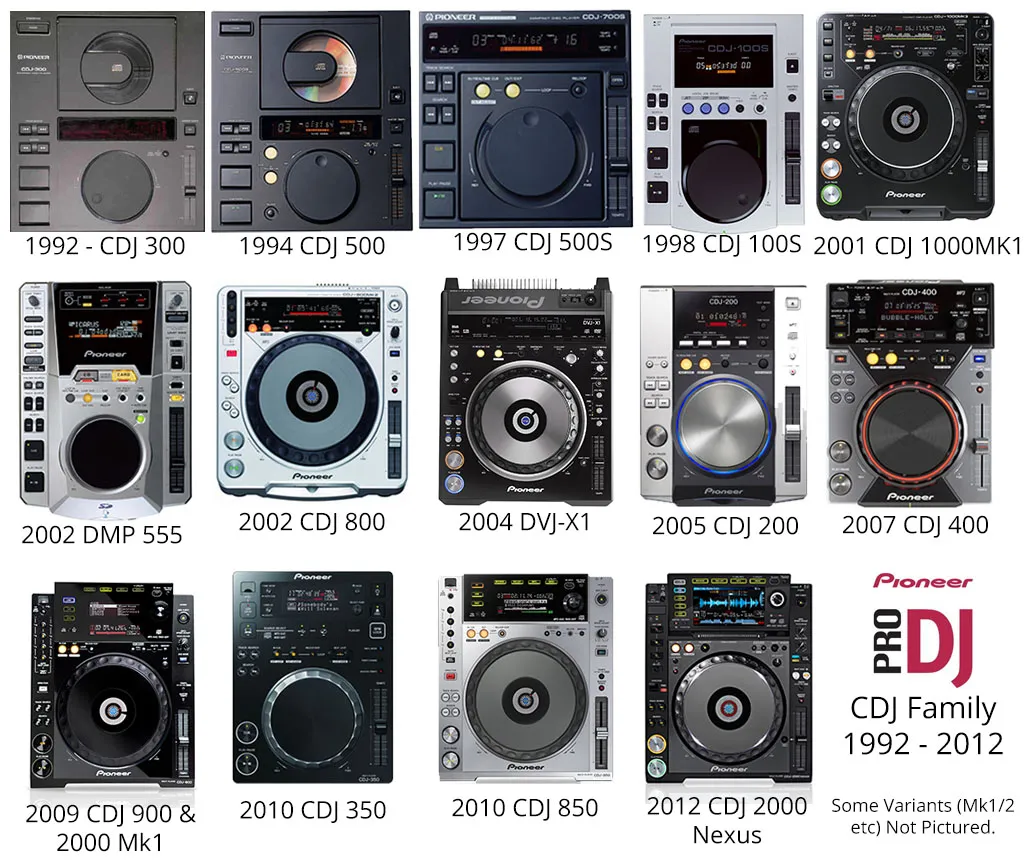
\includegraphics[scale=0.3]{images/pioneers_history}
	\centering
	\caption{Pioneer CDJ models from 1992-2012 \citep{chesters_history_2017}} 
\end{figure}

This chapter answers the following research question:
\\

\textit{Can a DJ-set centric dataset be used to solve other DJ tasks?} 
\\
\\
DJing (abbreviation of Disc Jockey) is a practice that has been the backbone of many sub cultures since the late 60s \citep{brewster_last_2014}. DJing has contributed to the evolution of various genres like Disco, Reggae, and the many forms of electronic dance music \citep{partridge_dub_2010, reynolds_energy_2013}. DJing traditionally involves two turntables and transitioning from one song to another in a stylised or fluid manner. The rise of digital audio during the 1990s saw the creation of CDJ's, and with it the introduction of mixing tool softwares such as Pioneer's rekordbox. Mixing tool software's makes use of music information retrieval techniques to lower the difficulty of organising and preparing for a DJ set \citep{kim_automatic_2017}. 

Music Information Retrieval is based on finding and compartmentalising the various aspects of music, including rhythm, timbre and melody \citep{orio_music_2006}. Implementations of music information retrieval vary from source separation and beat tracking. These tasks involve machine learning and deep learning algorithms, and are now fully embedded in DJ software \citep{rekordbox_rekordbox_2020}. 

\section{Source Separation}

Source separation involves estimating specific sources in one mixed signal \citep{jansson_singing_2017}. A music based example involves separating an instrument or voice within a track \citep{sgouros_efficient_2022}. Deep learning advancements have helped improve source separation in different fields. An example of this is U-nets, a convolutional neural network that proved effective in segmenting biomedical images \citep{ronneberger_u-net_2015}. With the use of spectrograms, a very similar model was used in a music source separation model \citep{jansson_singing_2017}. Deezer  further adapted this in their popular open source separator Spleeter \citep{hennequin_spleeter_2020}. Despite no published method, popular DJ manufacturer, Serato, released the Serato Stems update to there DJ software which provides similar functionality to Spleeter but in real time \citep{kirn_review_2023}. This has allowed DJs to make remixes in real time, separating instruments or voices from chosen songs.

As with most machine learning models, a rich dataset is essential for an application's accuracy \citep{jain_overview_2020}. The data used to trained for Jansson's U-Net model involved 20,000 track pairs of acapella and instrumental tracks \citep{jansson_singing_2017}. Isolated acapella or instrumental tracks are uncommon in DJ sets so the proposed model could not aid to further developments in source separation.


\section{BPM, key, genre classification}

\begin{figure}[H]
	
	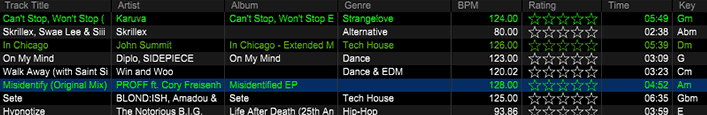
\includegraphics[scale=0.64]{images/rekordbox}
	\centering
	\caption{Playlist in rekordbox showing calculated BPM's and keys \citep{rekordbox_rekordbox_2023}} 
\end{figure}


Audio classification involves retrieving metadata from analysing an audio file \citep{sharma_audio_2021}. Audio classification models is used in DJ software's for calculating tempo, key and other musical attributes.

Despite increased popularity with deep learning, traditional machine learning techniques proves powerful enough for key detection. The Support Vector Machine proposed by George et. al had an accuracy value of 91.49\% and performed better compared to previous papers \citep{george_development_2022}. Support Vector Machine works well due its use of the kernel track and being able to handle linearity and non-linearity in data effectively \citep{hofmann_support_2006}. Having key information is essential within DJing because assuring the keys either match or modulate functionally assures fluidity in the transition. 

With tempo detection, Temporal Convolutional Networks are used effectively \citep{bock_deconstruct_2020}. Temporal Convolutional Networks are a hierarchy of temporal convolutions which can perform accurate detection and segmentation \citep{lea_temporal_2017}. The model was first used for tempo detection in 2019 \citep{bock_multi-task_2019}. The main breakthrough was the application  calculating the up beat and down beat, and through exploring both, each tasks saw increased accuracy from learning from the other \citep{bock_multi-task_2019}. When revisited in 2020, it was found that incorporating an extra dilation rate to each layer of the model gave more accurate results. Knowing the tempo of a given song is one of the main draws of CDJs over vinyl turntables, so further developments in tempo detection will inevitably find itself implemented in DJ software.

As the case for the BPM and key, recent advancements in genre classification have also ocurred. The most recent signification is a model that extracts short-time fourier transform, pitch, timbre and modified non-negative matrix factorisation features from a given piece of audio. These extractions are then fed through a deep belief neural network and optimised with a Wale Integreated sea lion algorithm \citep{kumaraswamy_optimal_2022}. A deep belief network is a generative model that uses stacks of restrictive Boltzmann machines (RBM) in its architecture \citep{canuma_what_2022}. The whale integrated sea lion algorithm is a nature inspired meta-heuristic optimisation algorithm that is good for advanced searches \citep{mirjalili_whale_2016}. Advancements in genre classification would be helpful within the DJ world as it would help the organisation of playlists for a given DJ.

Due to the dataset being built from DJ sets, it's unrealistic that the proposed method could compete with the classification methods discussed. However, a dataset built from DJ set could show audio examples of inputted songs being mixed.

\section{Automated Mixing}
Advances in classification and separation can automate preparation tasks for a DJ. However, there has also been deep learning advances that could all together replace a DJ. In February 2023, Spotify unravelled its brand new DJ feature. It combined situational music recommending accompanied by an AI generated host, mimicking the role of a personal broadcast DJ \citep{naomi_spotify_2023}. Within the research world, there have been advances on not just the mimicking of a human DJ's dialogue, but also the way in which a human would transition from one song to the next \citep{chen_automatic_2022}.

Spotify have had DJ style transitions and have ran experiments to show a general further appreciation to playlist that includes them \citep{bittner_automatic_2017}. In Bittner's  attempts to model DJ-style tranistions, peak detection is used to determine where-bout's in the song the "drops" occurs. Specific rules are given to assure appropriate drop in and drop out points for a given track \citep{bittner_automatic_2017}.  However Spotify's means of working out up and down beat was ineffective and greatly effected the fluidity of the transitions. A recent attempt found that using Boykov-Kolmogorov algorithm alongside spectrogram analysis of the two given songs made for great results for songs with similar tempos and keys \citep{robinson_automated_2023}. These models work with datasets very similar to the one in the proposed model. A fader estimation investigation ran in 2022 even uses MixesDB as a training dataset \citep{kim_joint_2022}. This indicates that a DJ-set centric dataset could be used to estimate parameter values during transitions from a dataset of DJ sets and audio files of songs in the tracklist.

\section{Summary}
An overview of DJing was given and how advancements in music information retrieval has helped its evolution. The recent technology behind Source separation, classification and automatic mixing was discussed. It was concluded that if the proposed model was developed further,useful information in regards to transitions could be found.

% note that \Blindocument has 5 numbered levels, despite setting secnumdepth above. I (and many style guides) would suggest using no more than 3 numbered levels (incl. the chapter), with the option of a fourth unnumbered level.